% !TEX program = xelatex
% Exam Cloner — CCF Computility 2026 答辩 PPT
\documentclass[aspectratio=169,11pt]{beamer}
\usepackage[UTF8]{ctex}
\usepackage{fontspec}
\usepackage{graphicx}
\usepackage{xcolor}
\usepackage{tikz}
\usetikzlibrary{positioning, arrows.meta, calc, fit, shapes.geometric, backgrounds}
\usepackage[most]{tcolorbox}

\IfFontExistsTF{Georgia}{\setmainfont{Georgia}}{}
\IfFontExistsTF{Noto Sans CJK SC}{\setsansfont{Noto Sans CJK SC}}{}

\definecolor{ivory}{HTML}{FAF9F6}
\definecolor{ivoryCard}{HTML}{FFFFFF}
\definecolor{ivoryWarm}{HTML}{F5F0E8}
\definecolor{ivoryDeep}{HTML}{EFE9DE}
\definecolor{ink}{HTML}{141413}
\definecolor{slateMuted}{HTML}{6B7280}
\definecolor{slateLight}{HTML}{9CA3AF}
\definecolor{coral}{HTML}{CC785C}
\definecolor{coralHover}{HTML}{B8654A}
\definecolor{success}{HTML}{16A34A}
\definecolor{warning}{HTML}{D97706}
\definecolor{border}{HTML}{E5E5E0}
\definecolor{borderSubtle}{HTML}{F0EDE6}

\setbeamertemplate{navigation symbols}{}
\setbeamertemplate{headline}{}
\setbeamercolor{background canvas}{bg=ivory}
\setbeamercolor{normal text}{fg=ink,bg=ivory}
\setbeamercolor{frametitle}{fg=ink,bg=ivory}
\setbeamercolor{itemize item}{fg=coral}
\setbeamercolor{enumerate item}{fg=coral}
\setbeamerfont{frametitle}{size=\Large,series=\bfseries}
\setbeamersize{text margin left=14mm,text margin right=14mm}
\setbeamertemplate{frametitle}{%
  \vspace{5mm}\begin{minipage}{\dimexpr\paperwidth-28mm\relax}
  {\usebeamerfont{frametitle}\insertframetitle}\par\vspace{1mm}
  {\color{coral}\rule{18mm}{1.2pt}}\end{minipage}\vspace{2mm}}
\setbeamertemplate{footline}{\hfill\textcolor{slateLight}{\scriptsize\insertframenumber\,/\,\inserttotalframenumber}\hspace{6mm}\vspace{3mm}}

\tcbset{%
  card/.style={enhanced,colback=ivoryCard,colframe=border,boxrule=.4pt,arc=2mm,left=4mm,right=4mm,top=3mm,bottom=3mm},
  warm/.style={enhanced,colback=ivoryWarm,colframe=borderSubtle,boxrule=.4pt,arc=2mm,left=4mm,right=4mm,top=2.5mm,bottom=2.5mm},
  accent/.style={enhanced,colback=coral!8,colframe=coral,boxrule=.6pt,arc=2mm,left=4mm,right=4mm,top=2.5mm,bottom=2.5mm}
}
\newcommand{\labeltext}[1]{{\scriptsize\color{slateMuted}\MakeUppercase{#1}}}
\newcommand{\coraltext}[1]{\textcolor{coral}{#1}}
\newcommand{\pill}[1]{\colorbox{ivoryWarm}{\scriptsize\strut\,#1\,}}
\title{Exam Cloner}
\subtitle{资源感知的 AI 考试备考系统}
\author{王语诺 \quad 刘睿淇}
\institute{香港科技大学（广州）}
\date{2026年7月24日 \quad·\quad CCF Computility 2026}

\begin{document}

% 1
\begin{frame}[plain]
  \begin{tikzpicture}[remember picture,overlay]
    \fill[coral] (current page.north west) rectangle ([xshift=6mm]current page.south west);
    \node[anchor=west] at ([xshift=18mm,yshift=-25mm]current page.north west) {\Huge\bfseries Exam Cloner};
    \node[anchor=west,text=slateMuted] at ([xshift=18mm,yshift=-37mm]current page.north west) {\Large 资源感知的 AI 考试备考系统};
    \node[anchor=west] at ([xshift=18mm,yshift=-55mm]current page.north west) {\large 王语诺 \quad 刘睿淇};
    \node[anchor=west,text=slateMuted] at ([xshift=18mm,yshift=-62mm]current page.north west) {\normalsize 香港科技大学（广州）};
    \node[anchor=west,text=slateLight,font=\small] at ([xshift=18mm,yshift=-75mm]current page.north west) {2026年7月24日 \quad·\quad CCF Computility 2026};
    \node[anchor=south east,text=slateMuted,font=\scriptsize] at ([xshift=-14mm,yshift=16mm]current page.south east) {CCF 算力网系统与应用大赛};
  \end{tikzpicture}
\end{frame}

% 2
\begin{frame}{一句话理解 Exam Cloner}
  \vspace{1mm}
  \begin{center}\Large
    把一堆课程材料，变成一条\coraltext{可持续的备考闭环}
  \end{center}
  \vspace{5mm}
  \begin{tikzpicture}[node distance=7mm and 6mm, every node/.style={align=center}]
    \tikzset{timelinebox/.style={draw=border,fill=ivoryCard,rounded corners=2mm,minimum width=27mm,minimum height=16mm,font=\small}, arrow/.style={-Stealth,very thick,draw=coral}}
    \node[timelinebox] (a) {上传材料\\{\scriptsize PDF / 作业 / 试卷}};
    \node[timelinebox,right=of a] (b) {解析与建库\\{\scriptsize 题目 / 知识点 / 风格}};
    \node[timelinebox,right=of b,fill=coral!10,draw=coral] (c) {练习与模拟\\{\scriptsize 自适应 + 风格克隆}};
    \node[timelinebox,right=of c] (d) {反馈回流\\{\scriptsize 批改 / 错题 / 复习}};
    \draw[arrow] (a)--(b); \draw[arrow] (b)--(c); \draw[arrow] (c)--(d);
    \draw[arrow,dashed] (d.south)
      .. controls ($(d.south)+(0,-14mm)$) and ($(c.south)+(0,-14mm)$) ..
      node[pos=.5,above=1mm,font=\tiny\color{slateMuted}] {错题回流} (c.south);
    \node[below=11mm of c,font=\scriptsize\color{slateMuted}] {每一步都看资源情况。能省的调用不发起，遇到故障也能继续};
  \end{tikzpicture}
  \vfill
  \begin{center}\scriptsize\pill{学习产品}\hspace{2mm}\pill{算力网应用}\hspace{2mm}\pill{真实部署}\end{center}
\end{frame}

% 3
\begin{frame}{备考有三个卡点，资源波动会把它们放大}
  \vspace{2mm}
  \begin{columns}[T]
    \column{.32\textwidth}\begin{tcolorbox}[card]
      \labeltext{材料}\par\vspace{2mm}{\large\bfseries 材料多，题目散}\par\vspace{2mm}
      \small 试卷、作业、课件各自孤立；知识点藏在 PDF 里，整理成本高。
    \end{tcolorbox}
    \column{.32\textwidth}\begin{tcolorbox}[card]
      \labeltext{反馈}\par\vspace{2mm}{\large\bfseries 刷题多，反馈浅}\par\vspace{2mm}
      \small 只知道对错，不知道缺了哪一步，也无法形成下一轮复习计划。
    \end{tcolorbox}
    \column{.32\textwidth}\begin{tcolorbox}[accent]
      \labeltext{算力}\par\vspace{2mm}{\large\bfseries 模型好，未必稳}\par\vspace{2mm}
      \small 限流、超时、无 GPU 都会让学习链路中断；单一模型依赖不可控。
    \end{tcolorbox}
  \end{columns}
  \vspace{5mm}\begin{center}\large\bfseries
    资源波动时，我们还能稳定地陪学生练下去吗？
  \end{center}
\end{frame}

% 4
\begin{frame}{解决方案把学习和算力接在一起}
  \vspace{2mm}
  \begin{center}
    \begin{tikzpicture}[node distance=5mm and 8mm]
      \tikzset{pillar/.style={draw=border,fill=ivoryCard,rounded corners=2mm,minimum width=32mm,minimum height=18mm,align=center,font=\small}, main/.style={draw=coral,fill=coral!10,rounded corners=2mm,minimum width=38mm,minimum height=20mm,align=center,font=\bfseries}}
      \node[pillar] (x) {材料解析\\{\scriptsize 结构化建库}};
      \node[main,right=of x] (y) {Exam Cloner\\{\scriptsize 学习闭环}};
      \node[pillar,right=of y] (z) {自适应复习\\{\scriptsize 按记忆情况安排间隔}};
      \node[pillar,below=of y] (r) {资源路由\\{\scriptsize 规则 / 题库 / 模型}};
      \draw[-Stealth,thick,draw=coral] (x)--(y)--(z); \draw[-Stealth,thick,draw=coral] (r)--(y);
    \end{tikzpicture}
  \end{center}
  \vspace{5mm}\begin{center}\small
    \pill{学习体验  风格克隆 · 五类题型批改 · 错题回流}\hspace{4mm}
    \pill{算力记录  路由理由 · 延迟 · fallback 轨迹}
  \end{center}
\end{frame}

% 5
\begin{frame}{系统架构，模型只是其中一环}
  \vspace{3mm}
  \begin{center}
  \resizebox{.96\textwidth}{!}{\begin{tikzpicture}[node distance=4mm and 6mm]
    \tikzset{box/.style={draw=border,fill=ivoryCard,rounded corners=1.5mm,minimum height=11mm,minimum width=31mm,align=center,font=\scriptsize}, core/.style={draw=coral,fill=coral!10,rounded corners=1.5mm,minimum height=13mm,minimum width=35mm,align=center,font=\small\bfseries}, arr/.style={-Stealth,thick,draw=slateMuted}}
    \node[box] (fe) {React + Vite\\学习工作台};
    \node[box,right=of fe] (be) {FastAPI + uv\\任务与数据};
      \node[core,right=of be] (router) {资源感知\\模型路由\\{\scriptsize 按资源情况选处理方式}};
    \node[box,above right=5mm and 6mm of router] (p1) {规则批改\\零算力};
    \node[box,right=6mm of router] (p2) {题库复用\\零算力};
    \node[box,below right=5mm and 6mm of router] (p3) {兼容模型\\DeepSeek / Ollama / vLLM};
    \node[box,below=8mm of router] (safe) {显式降级\\未批改，不误判};
    \draw[arr] (fe)--(be)--(router); \draw[arr] (router)--(p1); \draw[arr] (router)--(p2); \draw[arr] (router)--(p3); \draw[arr,dashed] (router)--(safe);
  \end{tikzpicture}}
  \end{center}
  \vspace{3mm}
  \begin{center}\scriptsize
    单进程部署 :3000 · JSON 原子存储 · SSRF 防护 · 浏览器侧密钥
  \end{center}
  \begin{center}\scriptsize\bfseries
    \coraltext{资源不可用时，产品能力下降，但学习流程不崩溃。}
  \end{center}
\end{frame}

% 6
\begin{frame}{创新一｜先省调用，再选模型}
  \vspace{2mm}
  \begin{columns}[T]
    \column{.58\textwidth}
    \begin{tikzpicture}[node distance=2.2mm]
      \tikzset{routerow/.style={draw=border,fill=ivoryCard,rounded corners=1mm,minimum width=74mm,minimum height=6mm,align=left,font=\scriptsize}, priorityrow/.style={routerow,draw=coral,fill=coral!10}}
      \node[priorityrow] (a) {01\quad{}规则批改，选择题和判断题本地完成};
      \node[priorityrow,below=of a] (b) {02\quad{}题库复用，已有题目不重复生成};
      \node[routerow,below=of b] (c) {03\quad{}用户选择的模型服务};
      \node[routerow,below=of c] (d) {04\quad{}管理员配置的本地服务};
      \node[routerow,below=of d] (e) {05\quad{}内置模型，必要时切换备用服务};
      \node[routerow,below=of e] (f) {06\quad{}没有服务时标记为未批改};
    \end{tikzpicture}
    \column{.38\textwidth}
    \begin{tcolorbox}[accent]
      \labeltext{算力网在这里做什么}\par\vspace{2mm}
      {\large\bfseries 资源有层级}\par\vspace{2mm}\scriptsize
      先走不花模型调用的路径。确实需要模型时，再从可用服务里选择。每个服务都有并发上限、超时和熔断保护。
    \end{tcolorbox}
    \vspace{2mm}
    \begin{tcolorbox}[warm]
      \centering\small\bfseries 3 次失败 → 熔断 60 秒\\[1mm]
      \scriptsize 遥测不记录密钥与完整 prompt
    \end{tcolorbox}
  \end{columns}
\end{frame}

% 7
\begin{frame}{创新二｜SM-2 让每次答题影响下一次复习}
  \vspace{3mm}
  \begin{center}
  \begin{tikzpicture}[node distance=13mm]
    \tikzset{n/.style={draw=border,fill=ivoryCard,rounded corners=2mm,minimum width=30mm,minimum height=15mm,align=center,font=\small}, c/.style={draw=coral,fill=coral!10,rounded corners=2mm,minimum width=34mm,minimum height=17mm,align=center,font=\small\bfseries}}
    \node[n] (q) {回答问题\\评分与反馈};
      \node[c,right=of q] (m) {更新掌握度\\难度系数};
    \node[n,right=of m] (d) {due-concept\\到期薄弱点};
    \node[n,below=of m] (nxt) {推送下一题\\调整难度};
    \draw[-Stealth,thick,draw=coral] (q)--(m)--(d); \draw[-Stealth,thick,draw=coral] (d)--(nxt)--(q);
  \end{tikzpicture}
  \end{center}
  \vspace{2mm}\begin{center}\scriptsize
    \pill{SM-2 按记忆情况安排复习间隔}\hspace{3mm}
    \pill{客观题即时反馈，主观题按需调用模型}
  \end{center}
\end{frame}

% 8
\begin{frame}{创新三｜照着原试卷出题，按步骤给反馈}
  \vspace{2mm}
  \begin{columns}[T]
    \column{.48\textwidth}\begin{tcolorbox}[card]
      {\Large\bfseries 试卷 → 风格画像}\par\vspace{3mm}
      \begin{tikzpicture}[node distance=3mm]
        \tikzset{mini/.style={draw=border,fill=ivoryWarm,rounded corners=1mm,minimum width=45mm,minimum height=7mm,align=center,font=\scriptsize}}
        \node[mini] (a) {从 PDF 提取文字和结构};\node[mini,below=of a] (b) {整理题型 / 难度 / 主题};\node[mini,below=of b] (c) {加入 3 道参考题，模仿原风格};\node[mini,below=of c,draw=coral,fill=coral!10] (d) {生成 80\% 题库 + 20\% 新题};
        \draw[-Stealth,draw=coral] (a)--(b)--(c)--(d);
      \end{tikzpicture}
    \end{tcolorbox}
    \column{.48\textwidth}\begin{tcolorbox}[accent]
      {\Large\bfseries 答案 → 结构化诊断}\par\vspace{3mm}\small
      系统会写清楚答案的问题和改法。\par\vspace{2mm}
      \pill{correct}\quad\pill{missing\_steps}\par\vspace{2mm}
      \pill{wrong\_concepts}\quad\pill{suggestion}\par\vspace{3mm}
      覆盖选择、判断、简答、计算、论述五类题型。
    \end{tcolorbox}
  \end{columns}
\end{frame}

% 9
\begin{frame}{算力中心里的真实路由记录}
  \vspace{1mm}
  \begin{center}
    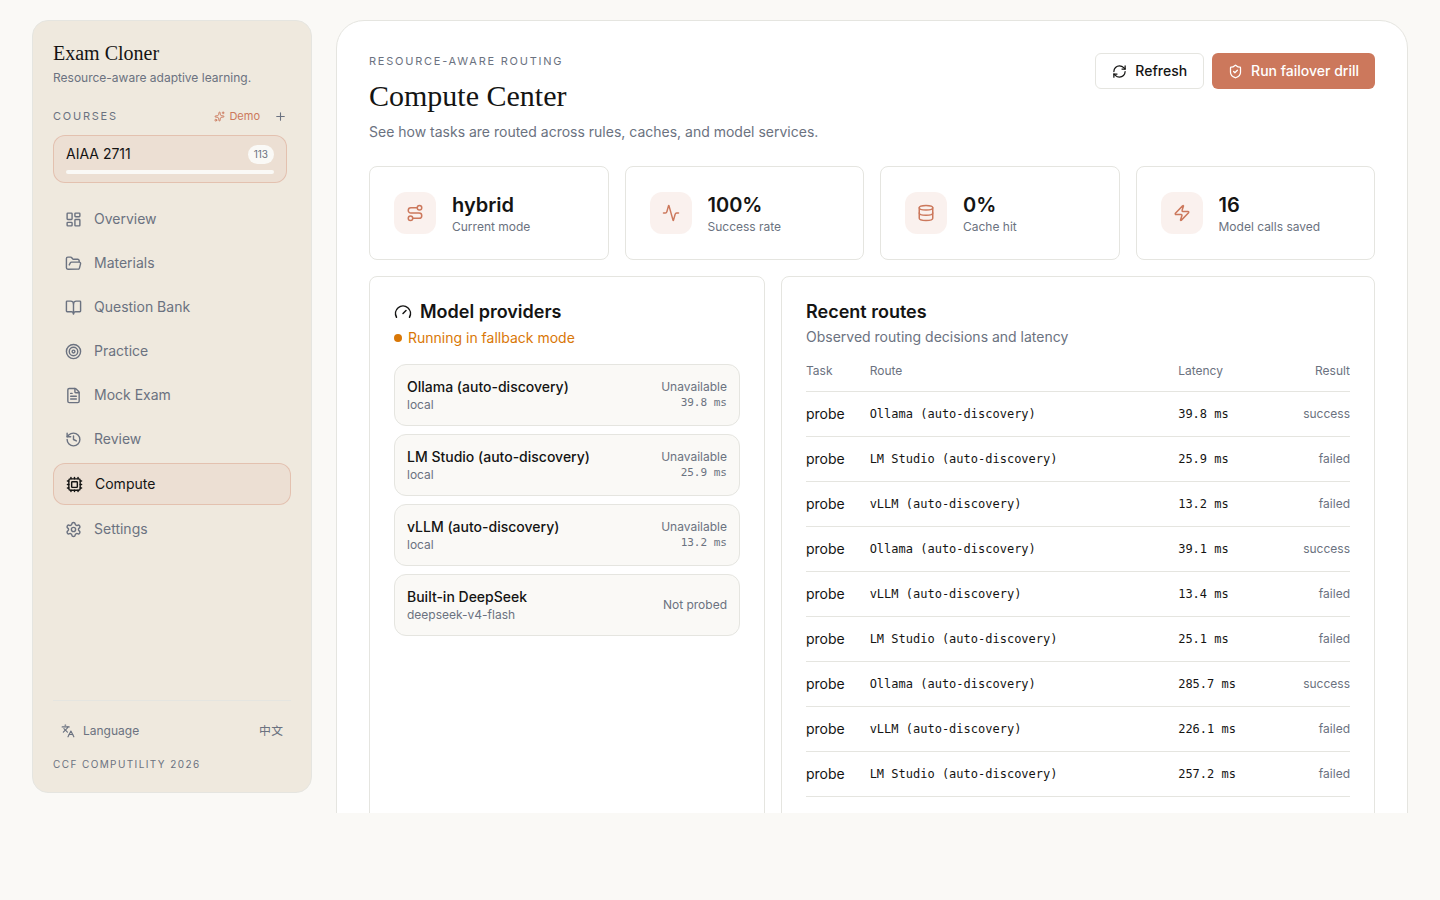
\includegraphics[width=.99\textwidth,height=.63\textheight,keepaspectratio]{assets/compute.png}
  \end{center}
  \vspace{0mm}\begin{center}\tiny\color{slateMuted}
    这里能看到服务状态、延迟、成功率、节省的模型调用和最近的路由轨迹
  \end{center}
\end{frame}

% 10
\begin{frame}{Dashboard 里直接看到下一步学习}
  \vspace{1mm}
  \begin{center}
    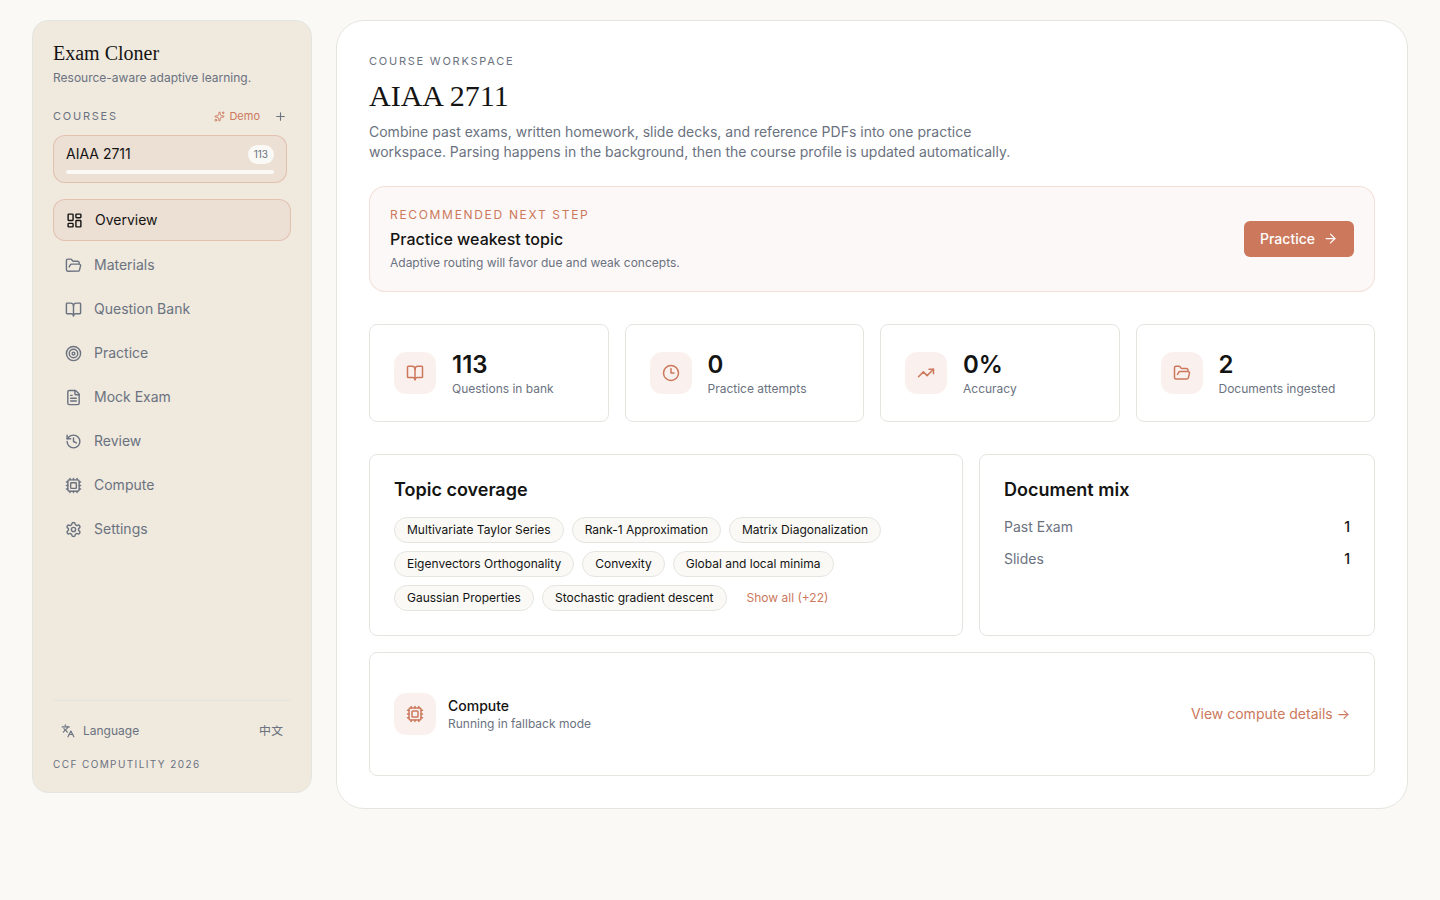
\includegraphics[width=.99\textwidth,height=.62\textheight,keepaspectratio]{assets/dashboard.png}
  \end{center}
  \vspace{0mm}\begin{center}\tiny\color{slateMuted}
    课程材料、题库规模、薄弱主题和推荐练习都在这里
  \end{center}
\end{frame}

% 11
\begin{frame}{现场演示走完一条学习路径}
  \vspace{1mm}
  \begin{center}
  \begin{tikzpicture}[node distance=6mm and 8mm]
    \tikzset{s/.style={draw=border,fill=ivoryCard,rounded corners=1.5mm,minimum width=38mm,minimum height=18mm,align=center,font=\small}, focus/.style={s,draw=coral,fill=coral!10}}
    \node[s] (a) {1\\载入演示课程};
    \node[s,right=of a] (b) {2\\查看算力中心};
    \node[focus,right=of b] (c) {3\\答客观题\\零算力};
    \node[focus,below=of a] (d) {4\\批改主观题\\看路由};
    \node[s,right=of d] (e) {5\\故障切换演练};
    \node[s,right=of e] (f) {6\\回 Dashboard\\看薄弱点};
    \draw[-Stealth,thick,draw=slateMuted] (a)--(b)--(c);
    \draw[-Stealth,thick,draw=slateMuted] (c.south) |- (d.north);
    \draw[-Stealth,thick,draw=slateMuted] (d)--(e)--(f);
  \end{tikzpicture}
  \end{center}
  \vspace{6mm}\begin{center}\small\color{slateMuted}\texttt{gpunion.hkust-gz.edu.cn/apps/exam-clone/}\end{center}
\end{frame}

% 12
\begin{frame}{工程细节让系统更稳}
  \vspace{3mm}
  \begin{columns}[T]
    \column{.24\textwidth}\begin{tcolorbox}[card]\centering {\LARGE\bfseries 3,082}\par\vspace{1mm}\scriptsize 后端业务源码行数\end{tcolorbox}
    \column{.24\textwidth}\begin{tcolorbox}[card]\centering {\LARGE\bfseries 3,711}\par\vspace{1mm}\scriptsize 前端 TypeScript 行数\end{tcolorbox}
    \column{.24\textwidth}\begin{tcolorbox}[card]\centering {\LARGE\bfseries 830}\par\vspace{1mm}\scriptsize 测试代码行数\end{tcolorbox}
    \column{.24\textwidth}\begin{tcolorbox}[accent]\centering {\LARGE\bfseries 0}\par\vspace{1mm}\scriptsize 未验收的 GPU 宣称\end{tcolorbox}
  \end{columns}
  \vspace{1mm}
  \begin{tcolorbox}[warm]
    \labeltext{正确性与安全}\par\vspace{1mm}\scriptsize
    所有权校验 · 幂等提交与错题导出 · 原子写入与线程锁 · 文件名消毒 · SSRF 与重定向校验 · 超时 / 熔断 / fallback 覆盖\par\vspace{2mm}
    \scriptsize GPU 执行保留接口与诊断能力；当前部署如实显示为 hardware acceptance pending。
  \end{tcolorbox}
\end{frame}

% 13
\begin{frame}{最后，我们交付了一套能学习也能看懂的系统}
  \vspace{4mm}
  \begin{columns}[T]
    \column{.32\textwidth}\begin{tcolorbox}[accent]\labeltext{01}\par\vspace{4mm}{\Large\bfseries 资源感知}\par\vspace{3mm}\small 规则、题库、模型分层路由；资源紧张也不中断。\end{tcolorbox}
    \column{.32\textwidth}\begin{tcolorbox}[card]\labeltext{02}\par\vspace{4mm}{\Large\bfseries 学习闭环}\par\vspace{3mm}\small 风格克隆、全题型批改、SM-2 复习调度连成一体。\end{tcolorbox}
    \column{.32\textwidth}\begin{tcolorbox}[card]\labeltext{03}\par\vspace{4mm}{\Large\bfseries 证据可见}\par\vspace{3mm}\small 路由、延迟、成功与节省调用都可在 Compute Center 验证。\end{tcolorbox}
  \end{columns}
  \vfill\begin{center}\small\color{slateMuted}
    接下来接入验收 GPU，支持图片和公式题，再把数据存储扩展到更多课程。
  \end{center}
\end{frame}

% 14
\begin{frame}[plain]
  \begin{tikzpicture}[remember picture,overlay]
    \fill[ink] (current page.north west) rectangle (current page.south east);
    \node[white] at (current page.center) {\begin{minipage}{.8\textwidth}\centering
      {\Huge\bfseries 谢谢！}\par\vspace{6mm}{\Large\color{ivoryWarm}欢迎提问与演示}\par\vspace{10mm}
      {\large\color{coral}Exam Cloner}\par\vspace{2mm}{\small\color{slateLight}王语诺 \;·\; 刘睿淇 \;·\; HKUST(GZ)}
    \end{minipage}};
  \end{tikzpicture}
\end{frame}
\end{document}
